\section{Vista de Casos de Uso}\label{sec:vista-casos-de-uso}

La Vista de Casos de Uso se centra en los aspectos funcionales de la plataforma. En esta vista se presentan los actores así como los casos de uso de la plataforma, y se detallan los casos de uso que se consideran críticos para la arquitectura \cite{LINS2026}.

\subsection{Actores}

\begin{itemize}
    \item \textbf{Público general y empresa cliente:} consulta información pública y valida permisos de empresas transportistas.
    \item \textbf{Ciudadano responsable de empresa:} administra el perfil de la empresa, vehículos, guías, viajes e infracciones.
    \item \textbf{Chofer:} consulta el viaje asignado y registra sus eventos desde la aplicación móvil.
    \item \textbf{Funcionario del MTOP:} gestiona empresas y fiscaliza permisos, vehículos, viajes, pesajes e infracciones.
    \item \textbf{Autoridad del MTOP:} consulta el tablero de indicadores y exporta reportes.
    \item \textbf{Administrador:} gestiona usuarios, roles, nodos periféricos y parámetros de fiscalización.
    \item \textbf{Usuario gub.uy:} autentica ciudadanos y funcionarios.
    \item \textbf{Plataforma de Interoperabilidad:} proporciona datos de ciudadanos mediante servicios de organismos públicos.
    \item \textbf{Sistema de Balanzas:} devuelve los pesajes de un vehículo para una fecha determinada.
    \item \textbf{Sistema de Tracking:} envía de forma continua las posiciones de los vehículos durante los viajes.
\end{itemize}

\subsection{Diagrama de Casos de Uso}

En esta sección se utilizan Diagramas de Casos de Uso UML para presentar los casos de uso de la plataforma, indicando cuáles se consideran críticos para la arquitectura. Los casos críticos son CU-01, CU-07, CU-09, CU-10, CU-11, CU-16 y CU-19; el CU-19 se incorporó a pedido del tutor por su complejidad.

\begin{figure}[H]
    \centering
    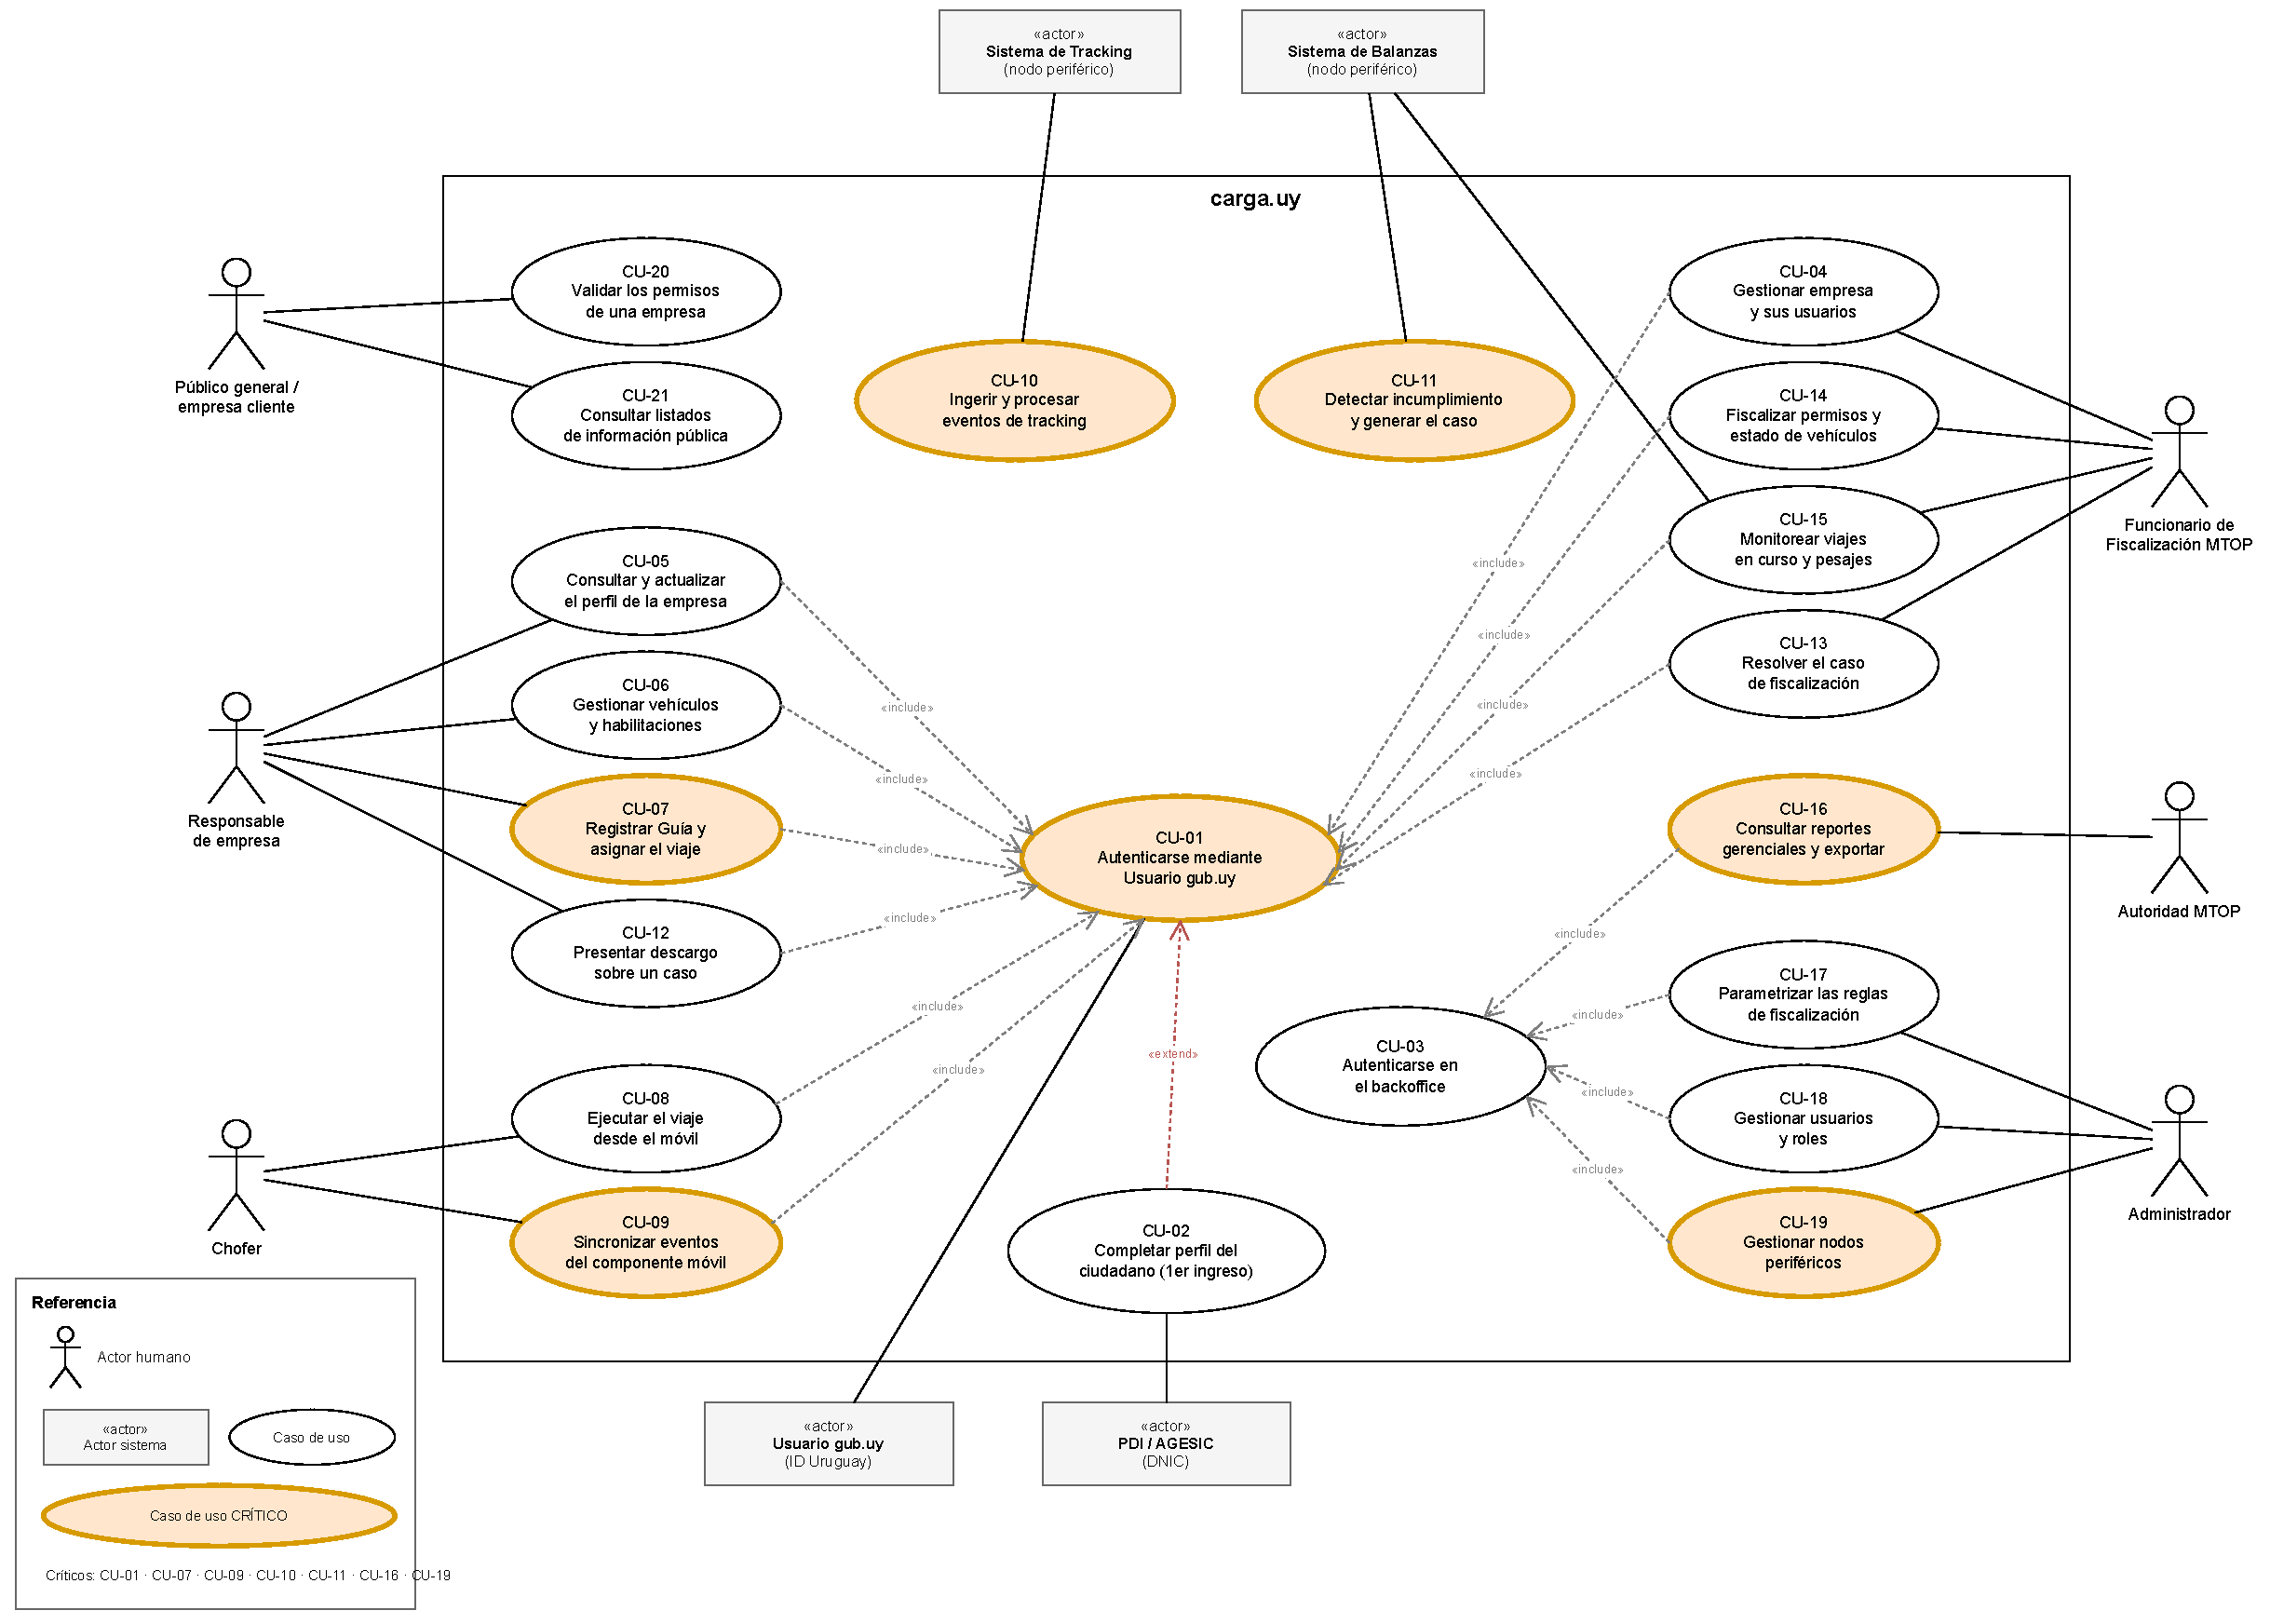
\includegraphics[width=\textwidth]{figures/casos-de-uso.pdf}
    \caption{Vista de Casos de Uso}
    \label{fig:usecases}
\end{figure}

La Tabla \ref{tab:cu-criticos} muestra qué componentes de la vista lógica (Sección \ref{sec:vista-logica}) intervienen en cada caso de uso crítico.

\begin{table}[H]
    \small
    \centering
    \caption{Componentes que intervienen en cada caso de uso crítico}
    \label{tab:cu-criticos}
    \begin{tabular}{|p{4.2cm}|p{11.6cm}|}
        \hline
        \textbf{Caso de uso} & \textbf{Componentes} \\
        \hline
        CU-01 Autenticarse mediante Usuario gub.uy & Frontoffice, API REST, Servicios de Negocio, Adaptador gub.uy, Persistencia y Usuario gub.uy. \\
        \hline
        CU-07 Registrar Guía y asignar el viaje & Frontoffice, Servicios de Negocio y Persistencia. \\
        \hline
        CU-09 Sincronizar los eventos del componente móvil & Componente Móvil y su persistencia local, API REST, Servicios de Negocio y Persistencia. \\
        \hline
        CU-10 Ingerir y procesar eventos de tracking & Nodo Periférico Tracking, Mensajería, Ingesta de Eventos, Persistencia y Motor de Fiscalización. \\
        \hline
        CU-11 Detectar un incumplimiento y generar el caso & Ingesta de Eventos, Motor de Fiscalización, Adaptador Balanzas, Nodo Periférico Balanzas, Persistencia, Notificaciones y Servicio de correo. \\
        \hline
        CU-16 Consultar reportes gerenciales y exportarlos & Backoffice, Generación de Reportes y Persistencia. \\
        \hline
        CU-19 Gestionar nodos periféricos & Backoffice, Servicios de Negocio y Persistencia; el registro de nodos condiciona además al Adaptador Balanzas y a la Ingesta de Eventos. \\
        \hline
    \end{tabular}
\end{table}

\pendiente{explicar el criterio con el que se eligieron los casos críticos. La plantilla propone dos: que intervenga el mayor número posible de componentes de la arquitectura y que intervengan los componentes críticos o más complejos.}

\FloatBarrier

\subsection{Funcionalidades Obligatorias}

\subsubsection{Frontoffice público}

\begin{enumerate}
    \item Autenticación mediante Usuario gub.uy.
    \item Validación de permisos de empresas transportistas.
    \item Consulta de listados de información pública agregada.
\end{enumerate}

\subsubsection{Frontoffice de empresas transportistas}

\begin{enumerate}
    \item \textbf{Perfil del ciudadano:} almacenar el correo electrónico y el número de cédula la primera vez que el usuario se autentica.
    \item \textbf{Perfil de la empresa:} consultar y actualizar nombre público, razón social, número de empresa y dirección principal.
    \item \textbf{Gestión de vehículos:} registrar matrícula, marca, modelo, peso, capacidad de carga, Permiso Nacional de Circulación e Inspección Técnica Vehicular.
    \item \textbf{Gestión de viajes:} ingresar guías con rubro del cliente, volumen, fecha, origen y destino, y asignarlas a un vehículo y un chofer.
    \item \textbf{Gestión de infracciones:} consultar infracciones y su evidencia, y presentar descargos dentro del plazo establecido.
\end{enumerate}

\subsubsection{Componente móvil}

\begin{enumerate}
    \item Autenticación mediante Usuario gub.uy.
    \item Consulta de la Guía y del viaje asignado al chofer.
    \item Registro del comienzo y finalización del viaje, cargas o descargas parciales e incidentes con fotografía opcional.
    \item Operación sin conectividad: la Guía debe estar disponible localmente; los eventos deben persistirse y sincronizarse al recuperar la conexión; cada evento debe tener un identificador generado en el dispositivo para evitar duplicados; y se debe definir una política de resolución de conflictos.
\end{enumerate}

\subsubsection{Frontoffice de funcionarios}

\begin{enumerate}
    \item Autenticación mediante Usuario gub.uy.
    \item Gestión de empresas de transporte.
    \item Fiscalización de permisos e ITV de los vehículos.
    \item Monitoreo de viajes en curso y finalizados, posiciones y pesajes.
    \item Gestión de casos de fiscalización: consultar evidencia y descargos, y confirmar o desestimar la infracción registrando el fundamento.
\end{enumerate}

\subsubsection{Backoffice de autoridades y administradores}

\begin{enumerate}
    \item Autenticación mediante un mecanismo interno y autorización basada en roles.
    \item Tablero para autoridades con cantidad de empresas y vehículos habilitados, viajes por período, volumen transportado por rubro, infracciones por tipo y tasa de confirmación.
    \item Filtrado de reportes por tipo de carga, ubicación y período, con exportación en al menos dos formatos.
    \item Gestión de usuarios, roles y nodos periféricos.
    \item Parametrización, sin redespliegue, de los umbrales de exceso de carga y desvío de ruta.
\end{enumerate}

\subsection{Fiscalización Automática}

La plataforma debe detectar como mínimo:

\begin{itemize}
    \item \textbf{Exceso de carga:} el pesaje supera el peso del vehículo más su capacidad declarada.
    \item \textbf{Vehículo sin habilitación vigente:} el permiso o la ITV están vencidos a la fecha del viaje.
    \item \textbf{Viaje sin Guía:} se recibe tracking o un pesaje para un vehículo sin un viaje asignado y en curso.
    \item \textbf{Desvío de ruta:} el recorrido reportado se aparta significativamente del trayecto esperado entre el origen y el destino declarados.
\end{itemize}

Cada detección genera un caso cuyo ciclo de vida es \emph{detectada}, \emph{notificada}, \emph{en descargo} y, finalmente, \emph{confirmada} o \emph{desestimada}. La detección debe ser automática y asincrónica; las transiciones deben estar controladas; la empresa debe ser notificada; las acciones de los funcionarios deben quedar auditadas; y el reprocesamiento de un evento no debe crear casos duplicados.

\FloatBarrier

\subsection{Casos de Uso Críticos}

Cada caso de uso crítico se describe en una de las siguientes subsecciones, con su descripción, sus precondiciones, el flujo principal, los flujos alternativos relevantes y sus postcondiciones.

\subsubsection{CU-01 Autenticarse mediante Usuario gub.uy}\label{sec:cu-01}
\begin{table}[H]
\small
\setlength{\tabcolsep}{8pt}
\renewcommand{\arraystretch}{1.1}
\centering
\begin{tabular}{|p{15.8cm}|}
\hline
\textbf{\underline{Actor principal:}} Ciudadano (responsable o chofer) o Funcionario MTOP. \\ \hline
\textbf{\underline{Actor secundario:}} Usuario gub.uy (ID Uruguay). \\ \hline
\textbf{\underline{Canales:}} Frontoffice web y componente móvil. \\ \hline
\textbf{\underline{Descripción:}} Permite que el usuario se identifique mediante Usuario gub.uy. Una vez autenticado, carga.uy crea la sesión y determina los permisos que le corresponden. \\ \hline
\textbf{\underline{Precondición:}} El usuario posee un Usuario gub.uy vigente. \\ \hline
\textbf{\underline{Flujo principal:}}\par
\begin{enumerate}[leftmargin=*,topsep=2pt,itemsep=1pt,parsep=0pt,partopsep=0pt]
    \item El usuario solicita ingresar.
    \item El sistema lo redirige a Usuario gub.uy.
    \item El usuario completa la autenticación.
    \item Usuario gub.uy devuelve el resultado.
    \item El sistema valida la respuesta y obtiene cédula y correo.
    \item Busca un perfil local asociado a la cédula.
    \item Establece la sesión, resuelve roles y permisos, y redirige al usuario.
    \item Registra el ingreso con identificador de correlación.
\end{enumerate} \\ \hline
\textbf{\underline{Alternativas y excepciones:}}\par
\begin{itemize}[leftmargin=*,topsep=2pt,itemsep=1pt,parsep=0pt,partopsep=0pt]
    \item Si no existe perfil local, se crea antes de establecer la sesión.
    \item Un ciudadano sin empresa asociada accede solamente a funciones públicas.
    \item Una autenticación cancelada, fallida, inválida o vencida no crea sesión.
    \item Si gub.uy no responde, las funcionalidades públicas siguen disponibles.
    \item En el móvil, una sesión previa válida permite operar sin conexión.
\end{itemize} \\ \hline
\textbf{\underline{Postcondiciones:}} Existe una sesión con identidad, roles y permisos resueltos, o no existe sesión. El evento queda registrado y no se almacenan credenciales del usuario. \\ \hline
\end{tabular}
\end{table}

\subsubsection{CU-07 Registrar Guía y asignar el viaje}\label{sec:cu-07}
\begin{table}[H]
\small
\setlength{\tabcolsep}{8pt}
\renewcommand{\arraystretch}{1.1}
\centering
\begin{tabular}{|p{15.8cm}|}
\hline
\textbf{\underline{Actor principal:}} Responsable de empresa. \\ \hline
\textbf{\underline{Descripción:}} Permite registrar la Guía de un viaje de carga y asignarla a un vehículo y a un chofer de la empresa. \\ \hline
\textbf{\underline{Precondiciones:}} El responsable está autenticado, la empresa está activa y existen al menos un vehículo y un chofer disponibles. \\ \hline
\textbf{\underline{Flujo principal:}}\par
\begin{enumerate}[leftmargin=*,topsep=2pt,itemsep=1pt,parsep=0pt,partopsep=0pt]
    \item El responsable selecciona “nueva Guía”.
    \item Ingresa rubro, volumen y tipo de carga, fecha, origen y destino.
    \item El sistema valida los datos y calcula el recorrido esperado.
    \item Genera una Guía única en estado \emph{registrada}.
    \item El responsable selecciona un vehículo habilitado y un chofer.
    \item El sistema valida que no existan viajes solapados.
    \item Crea el viaje en estado \emph{asignado} y lo publica en el móvil.
    \item Notifica al chofer.
\end{enumerate} \\ \hline
\textbf{\underline{Alternativas y excepciones:}}\par
\begin{itemize}[leftmargin=*,topsep=2pt,itemsep=1pt,parsep=0pt,partopsep=0pt]
    \item Se rechaza la asignación si el Permiso o la ITV no están vigentes.
    \item Se rechaza si la capacidad del vehículo es insuficiente o existe un solapamiento.
    \item Un origen o destino no georreferenciable debe corregirse.
    \item Una cancelación previa al inicio deja el viaje en estado \emph{cancelado}.
\end{itemize} \\ \hline
\textbf{\underline{Postcondiciones:}} Existe una Guía con viaje, vehículo, chofer y recorrido esperado. El viaje queda disponible para el chofer y sirve como referencia para tracking y pesajes. \\ \hline
\end{tabular}
\end{table}

\subsubsection{CU-09 Sincronizar los eventos del componente móvil}\label{sec:cu-09}
\begin{table}[H]
\small
\setlength{\tabcolsep}{8pt}
\renewcommand{\arraystretch}{1.1}
\centering
\begin{tabular}{|p{15.8cm}|}
\hline
\textbf{\underline{Actor principal:}} Chofer. \\ \hline
\textbf{\underline{Descripción:}} Sincroniza los eventos registrados sin conexión, evita duplicados y trata los conflictos producidos si el viaje cambió mientras el dispositivo estaba fuera de línea. \\ \hline
\textbf{\underline{Precondiciones:}} Existen eventos pendientes, se recuperó la conectividad y la sesión está vigente o pudo renovarse. \\ \hline
\textbf{\underline{Flujo principal:}}\par
\begin{enumerate}[leftmargin=*,topsep=2pt,itemsep=1pt,parsep=0pt,partopsep=0pt]
    \item La aplicación ordena y envía los eventos pendientes con sus identificadores.
    \item El componente central verifica si cada identificador ya fue procesado.
    \item Aplica los eventos nuevos respetando la máquina de estados.
    \item Descarta los eventos conocidos sin repetir sus efectos.
    \item Responde con el resultado y la versión actual del viaje.
    \item La aplicación elimina de la cola los eventos confirmados.
\end{enumerate} \\ \hline
\textbf{\underline{Alternativas y excepciones:}}\par
\begin{itemize}[leftmargin=*,topsep=2pt,itemsep=1pt,parsep=0pt,partopsep=0pt]
    \item Los eventos de un viaje cancelado o reasignado se conservan como evidencia y se marca el conflicto.
    \item Los eventos no confirmados se reenvían si la sincronización se interrumpe.
    \item Ante recuperaciones simultáneas de conectividad, los eventos permanecen pendientes hasta poder procesarse.
\end{itemize} \\ \hline
\textbf{\underline{Postcondiciones:}} Cada evento produce un único efecto; no existen duplicados y los conflictos quedan marcados sin pérdida de información. \\ \hline
\end{tabular}
\end{table}

\subsubsection{CU-10 Ingerir y procesar eventos de tracking}\label{sec:cu-10}
\begin{table}[H]
\small
\setlength{\tabcolsep}{8pt}
\renewcommand{\arraystretch}{1.1}
\centering
\begin{tabular}{|p{15.8cm}|}
\hline
\textbf{\underline{Actor principal:}} Sistema de Tracking (nodo periférico). \\ \hline
\textbf{\underline{Descripción:}} Recibe las posiciones enviadas por los vehículos durante un viaje y las utiliza para reconstruir la ruta recorrida. \\ \hline
\textbf{\underline{Precondiciones:}} El nodo de tracking está registrado y habilitado, y el mecanismo de mensajería está disponible. \\ \hline
\textbf{\underline{Flujo principal:}}\par
\begin{enumerate}[leftmargin=*,topsep=2pt,itemsep=1pt,parsep=0pt,partopsep=0pt]
    \item El nodo publica eventos con vehículo, coordenadas, marca de tiempo e identificador.
    \item El componente central recibe y encola los eventos.
    \item Un consumidor toma los eventos de la cola.
    \item Descarta los identificadores ya procesados.
    \item Asocia cada evento al viaje que estaba en curso cuando se generó.
    \item Ordena las posiciones por su momento de generación.
    \item Actualiza las métricas de procesamiento.
\end{enumerate} \\ \hline
\textbf{\underline{Alternativas y excepciones:}}\par
\begin{itemize}[leftmargin=*,topsep=2pt,itemsep=1pt,parsep=0pt,partopsep=0pt]
    \item Un vehículo sin viaje en curso al generarse el evento dispara la regla \emph{viaje sin Guía}.
    \item Ante saturación, los eventos permanecen encolados y pueden agregarse consumidores.
    \item Si el nodo no responde, el componente central continúa funcionando.
    \item Los eventos tardíos se incorporan a la ruta histórica y vuelven a evaluar las reglas.
\end{itemize} \\ \hline
\textbf{\underline{Postcondiciones:}} La ruta contiene las posiciones recibidas, ordenadas y sin duplicados, sin pérdida dentro del volumen objetivo. \\ \hline
\end{tabular}
\end{table}

\textbf{Asociación de posiciones a viajes.} Cada posición se asocia al viaje que el vehículo tenía en curso a la hora en que se generó la posición, y no al que tiene cuando la posición llega al componente central. Las horas de inicio y fin de cada viaje son las que registró el chofer en la aplicación móvil.

Por ejemplo, si un viaje va de 10:00 a 12:00 y el vehículo pierde cobertura desde las 11:30, las posiciones de 11:30 a 12:00 pueden llegar a las 12:15, con el viaje ya finalizado. Con este criterio igual quedan en ese viaje. Si se mirara el estado del viaje al llegar cada posición, parecerían de un vehículo sin viaje y se abriría un caso falso de \emph{viaje sin Guía}.

Puede pasar también lo inverso: si el chofer inicia el viaje sin conexión, las posiciones llegan antes que el aviso de inicio. Cuando el aviso llega, esas posiciones se asocian al viaje y se vuelve a evaluar la regla \emph{viaje sin Guía}.

\subsubsection{CU-11 Detectar automáticamente un incumplimiento y generar el caso}\label{sec:cu-11}
\begin{table}[H]
\small
\setlength{\tabcolsep}{8pt}
\renewcommand{\arraystretch}{1.1}
\centering
\begin{tabular}{|p{15.8cm}|}
\hline
\textbf{\underline{Disparador:}} El procesamiento de un evento de tracking (CU-10) o del fin de un viaje registrado desde el móvil (CU-09); no tiene actor humano. \\ \hline
\textbf{\underline{Actores secundarios:}} Sistema de Balanzas y empresa transportista. \\ \hline
\textbf{\underline{Descripción:}} Cruza la información declarada con los datos de tracking y balanzas para detectar incumplimientos y generar el caso correspondiente. \\ \hline
\textbf{\underline{Precondiciones:}} Existen datos declarados y recibidos, y los umbrales de tolerancia están parametrizados. \\ \hline
\textbf{\underline{Flujo principal:}}\par
\begin{enumerate}[leftmargin=*,topsep=2pt,itemsep=1pt,parsep=0pt,partopsep=0pt]
    \item La detección se ejecuta en segundo plano.
    \item Si el evento es el fin de un viaje, consulta a Balanzas los pesajes del vehículo y evalúa el exceso de carga.
    \item Verifica la vigencia del Permiso y la ITV.
    \item Detecta actividad de vehículos sin Guía.
    \item Compara la ruta con el recorrido y los umbrales configurados.
    \item Comprueba que el hecho no haya generado otro caso.
    \item Crea el caso en estado \emph{detectada} y almacena la evidencia.
    \item Lo publica y solicita la notificación a la empresa; al confirmarse el envío, el caso pasa a \emph{notificada} e inicia el plazo de descargo.
    \item Registra la creación en la pista de auditoría.
\end{enumerate} \\ \hline
\textbf{\underline{Alternativas y excepciones:}}\par
\begin{itemize}[leftmargin=*,topsep=2pt,itemsep=1pt,parsep=0pt,partopsep=0pt]
    \item Si Balanzas no responde, la evaluación queda pendiente sin detener la plataforma.
    \item La evidencia nueva se agrega a un caso existente por el mismo hecho.
    \item No se determina un desvío con posiciones insuficientes.
    \item Una falla del correo no bloquea el caso y provoca un reintento.
\end{itemize} \\ \hline
\textbf{\underline{Postcondiciones:}} Existe un caso con evidencia, en estado \emph{notificada} o en \emph{detectada} hasta que se confirme el envío, sin duplicados y con su creación auditada. \\ \hline
\end{tabular}
\end{table}

\textbf{Consulta a balanzas.} La integración con balanzas es de solicitud--respuesta (R3): los pesajes no llegan solos, el componente central los pide por vehículo y fecha. Por eso el exceso de carga se evalúa cuando el viaje finaliza: el motor pide los pesajes de cada fecha del viaje y compara cada pesada del horario del viaje con el peso del vehículo más su capacidad declarada. La justificación está en la decisión DA10 (Tabla \ref{tab:da10}).

\subsubsection{CU-16 Consultar reportes gerenciales y exportarlos}\label{sec:cu-16}
\begin{table}[H]
\small
\setlength{\tabcolsep}{8pt}
\renewcommand{\arraystretch}{1.1}
\centering
\begin{tabular}{|p{15.8cm}|}
\hline
\textbf{\underline{Actor principal:}} Autoridad MTOP. \\ \hline
\textbf{\underline{Descripción:}} Permite consultar indicadores generales de operación y fiscalización, aplicar filtros y exportar los resultados. \\ \hline
\textbf{\underline{Precondición:}} La autoridad está autenticada en el backoffice con el rol correspondiente. \\ \hline
\textbf{\underline{Flujo principal:}}\par
\begin{enumerate}[leftmargin=*,topsep=2pt,itemsep=1pt,parsep=0pt,partopsep=0pt]
    \item La autoridad accede al dashboard.
    \item El sistema presenta los indicadores obligatorios.
    \item La autoridad filtra por carga, ubicación y período.
    \item El sistema recalcula los indicadores.
    \item La autoridad solicita una exportación en CSV o PDF.
    \item El sistema genera el archivo y lo pone a disposición.
\end{enumerate} \\ \hline
\textbf{\underline{Alternativas y excepciones:}}\par
\begin{itemize}[leftmargin=*,topsep=2pt,itemsep=1pt,parsep=0pt,partopsep=0pt]
    \item Un rango muy amplio genera una advertencia o una limitación del período.
    \item Una exportación grande se genera en segundo plano.
    \item Si no existen datos, se informa explícitamente.
    \item El umbral de agregación pública no limita los reportes internos del MTOP.
\end{itemize} \\ \hline
\textbf{\underline{Postcondiciones:}} La autoridad visualizó los indicadores y, si corresponde, obtuvo el archivo. El acceso quedó registrado. \\ \hline
\end{tabular}
\end{table}

\subsubsection{CU-19 Gestionar nodos periféricos}\label{sec:cu-19}
\begin{table}[H]
\small
\setlength{\tabcolsep}{8pt}
\renewcommand{\arraystretch}{1.1}
\centering
\begin{tabular}{|p{15.8cm}|}
\hline
\textbf{\underline{Actor principal:}} Administrador. \\ \hline
\textbf{\underline{Actores secundarios:}} Nodo Periférico Balanzas y Nodo Periférico Tracking. \\ \hline
\textbf{\underline{Canales:}} Backoffice web. \\ \hline
\textbf{\underline{Descripción:}} Permite registrar, consultar, modificar, habilitar, deshabilitar y dar de baja los nodos periféricos de balanzas y de tracking de los que la plataforma obtiene pesajes y posiciones. \\ \hline
\textbf{\underline{Precondiciones:}} El administrador está autenticado en el backoffice con el rol correspondiente y el componente periférico está desplegado. \\ \hline
\textbf{\underline{Flujo principal:}}\par
\begin{enumerate}[leftmargin=*,topsep=2pt,itemsep=1pt,parsep=0pt,partopsep=0pt]
    \item El administrador accede a la gestión de nodos y el sistema lista los nodos registrados con su tipo, punto de acceso y estado.
    \item Selecciona registrar un nodo e indica su tipo (balanzas o tracking), un identificador y su punto de acceso.
    \item El sistema valida que el identificador no esté en uso.
    \item Registra el nodo en estado \emph{deshabilitado}.
    \item El administrador solicita verificar la conectividad con el nodo.
    \item Si la verificación es exitosa, el administrador habilita el nodo.
    \item A partir de ese momento el nodo intercambia datos con el componente central.
\end{enumerate} \\ \hline
\textbf{\underline{Alternativas y excepciones:}}\par
\begin{itemize}[leftmargin=*,topsep=2pt,itemsep=1pt,parsep=0pt,partopsep=0pt]
    \item Si el identificador ya está en uso, se rechaza el registro.
    \item Si la verificación falla, el nodo permanece deshabilitado y se informa el motivo.
    \item Modificar el punto de acceso de un nodo habilitado lo vuelve a \emph{deshabilitado} hasta una nueva verificación.
    \item Deshabilitar un nodo de balanzas deja pendiente la evaluación de exceso de carga sin detener la plataforma.
    \item Deshabilitar un nodo de tracking hace que se descarten sus eventos y los viajes en curso quedan sin actualización de ruta.
    \item La baja es lógica: los pesajes y las posiciones que el nodo reportó siguen siendo evidencia de los casos generados.
\end{itemize} \\ \hline
\textbf{\underline{Postcondiciones:}} El nodo queda registrado con su tipo, punto de acceso y estado. Solo los nodos habilitados intercambian datos con el componente central y ninguna credencial queda en el repositorio. \\ \hline
\end{tabular}
\end{table}

La verificación de conectividad consulta el punto de acceso del nodo: a un nodo de balanzas se le hace una consulta de pesajes de prueba, y a un nodo de tracking se le consulta su estado (\texttt{/health}), que indica si está conectado a la mensajería.
